\documentclass[10pt,a4paper]{article}
\usepackage[utf8x]{inputenc}
\usepackage[danish]{babel}
\usepackage{amsmath}
\usepackage{mathtools}
\usepackage{framed}
\usepackage{amsfonts}
%\usepackage{hyperref}
\usepackage{todonotes}
\usepackage{float}
\usepackage{amssymb}
\setlength{\parindent}{0pt}
\usepackage{graphicx}
\usepackage{fullpage}
\DeclarePairedDelimiter\ceil{\lceil}{\rceil}
\DeclarePairedDelimiter\floor{\lfloor}{\rfloor}
\newcount\colveccount
\newcommand*\colvec[1]{
        \global\colveccount#1
        \begin{pmatrix}
        \colvecnext
}
\def\colvecnext#1{
        #1
        \global\advance\colveccount-1
        \ifnum\colveccount>0
                \\
                \expandafter\colvecnext
        \else
                \end{pmatrix}
        \fi
}

\title{Exercise 4: Naïve Bayes classification}
\author{Group 2: Keerthikan Ratnarajah \& Mikael Westermann}


\begin{document}
\maketitle

\section{Näives Bayes method}
Naive bayes method is a classification algorithm based on bayes rule and a set independence features. The naive bayes classifier assumes that the presence of a particular feature in a class is unrelated to the presence of any other feature, which often is not the case. 

\begin{figure}[H]
\centering
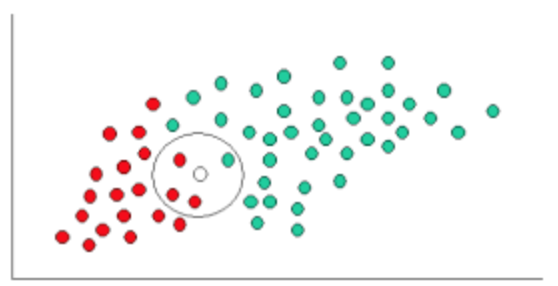
\includegraphics[width = 0.4\textwidth]{image.png}
\end{figure}


To demonstrate the concept of naive bayes classifcation consider the example illustrated in figure. 
The object depicted in the figure above belongs either the class green or red.  The task of the classifier is to classify new  observations and decide whether it belong to the class red or green. \\

Using bayes is this possible, first is the prior probability determined. In this case is it very likely to believe that a new obersevation would belong to the class green, since the amount green balls is larger than red.  The beliefs is known as the prior probability, is the probability based on prior experience. 

\begin{equation}
\centering
P(green) = \frac{number~of~green}{total~number~of~object}
\end{equation}

\begin{equation}
\centering
P(red) = \frac{number~of~red}{total~number~of~object}
\end{equation}

Using the prior probability, Will  a new object be classified. 

\begin{figure}[H]
\centering
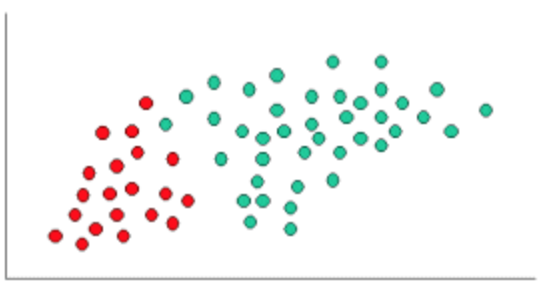
\includegraphics[width = 0.4\textwidth]{image2.png}
\end{figure}
The likelihood of the object either belonging to the class red or class green is completely determined by the object lying near it. 

\begin{equation}
\centering
likelihood~of~object~being~green = \frac{Number~of~green~in~the~vicinity~of~the~new~object }{total~number~of~green~object}
\end{equation}

\begin{equation}
\centering
likelihood~of~object~being~red = \frac{Number~of~red~in~the~vicinity~of~the~new~object }{total~number~of~red~object}
\end{equation}


In a bayesian analysis is the final classification produced by combining the prior and the likelihood information, to form the posterior probability, using the bayes rule . 


Formally can this be written as 
\begin{equation}
\centering
P(c|x) = \frac{P(x|c)P(c)}{P(x)}
\end{equation}

where 
\begin{itemize}
\item	$p(c|x)$ is the posterior probability of class given observation x
\item	$p(c)$ is the prior probability of class
\item   $p(x|c)$ is the likelihood which observation belongs to class  c
\item   $p(x)$ is the prior probability of the observation. 
\end{itemize}

%\todo[inline]{https://documents.software.dell.com/statistics/textbook/naive-bayes-classifier}




 

\section{Analysis}
Since the dataset consisting of the raw data is a contionous dataset, one have to be binned before they can be processed. Binning is a way of dicretization the data in to numerical variables into categorical counterparts. The binary data were binned based on interval sizes.  A small intervall size would create a large amount bins categories and a large intervall would create a small amount of bin category.  

First were the model created with different number of bins from a dataset consisting one person, and then tested with another dataset.

\begin{figure}[H] 
\centering
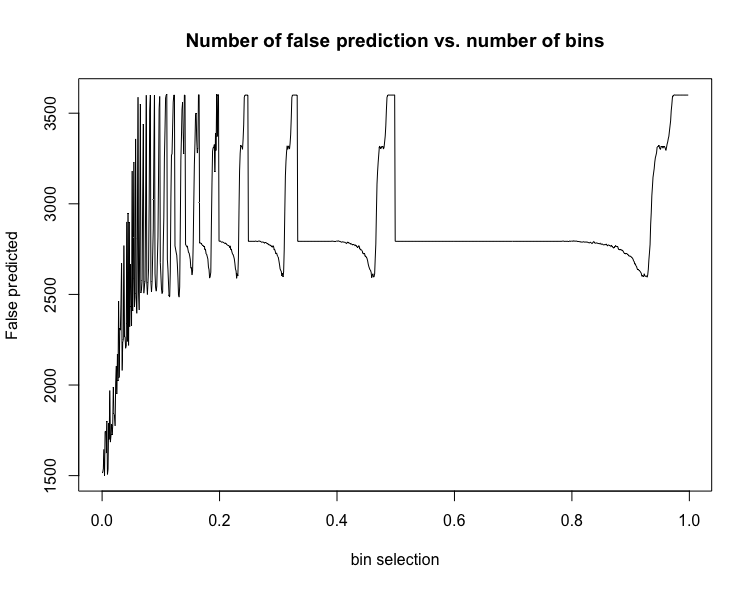
\includegraphics[width = \textwidth]{number_of_false_prediction_vs_number_of_bins_plot.png}
\label{fig:false_g_g}
\caption{Graph showing amount false prediction vs. interval size of the bins}
\end{figure}

Based from the figure \ref{fig:false_g_g}, could it be seen that  the amount of false prediction computed were dependent of the number of bins, which makes sense as the variabillity of the data changes, based on this observation were same test peformed for the whole class vs. one person who was not part of the complete dataset. 

\begin{figure}[H]
\centering
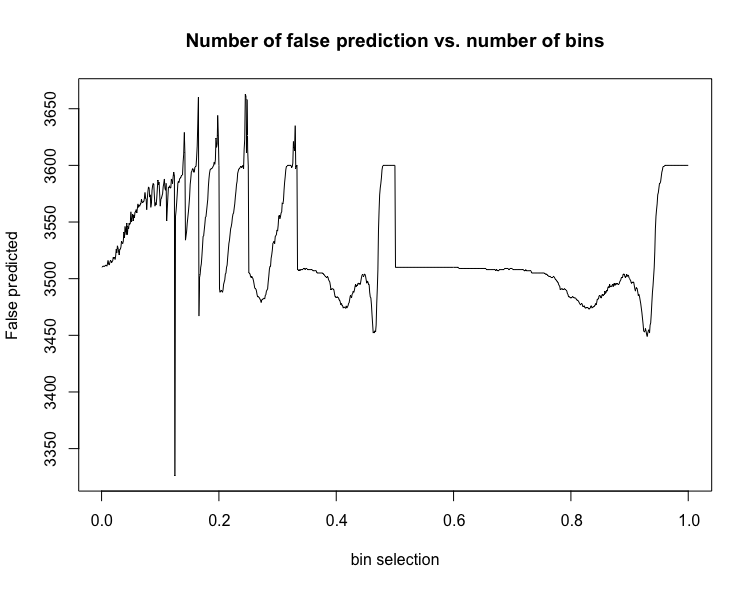
\includegraphics[width = \textwidth]{g2M2vsFewer.png}
\label{fig:false_g_f}
\caption{Graph showing amount palse precidiction vs. interval size of the bins}
\end{figure}

The dataset used for testing entailed  4000 observation, which the previous one also had but comparing the the them both shows that the result of increasing the amount of training make the prediction worse, which wasnt the case before.

Looking at the confusion matrix from the iterations shows this

\begin{figure}[!htb]
\minipage{0.32\textwidth}
  \includegraphics[width=\linewidth]{confus_10.eps}
\label{fig:awesome_image1}
\caption{bin selection - 0.010}
\endminipage\hfill
\minipage{0.32\textwidth}
  \includegraphics[width=\linewidth]{confus_32.eps}
\label{fig:awesome_image2}
\caption{bin selection - 0.032}
\endminipage\hfill
\minipage{0.32\textwidth}%
  \includegraphics[width=\linewidth]{confus_62.eps}
 \label{fig:awesome_image3}
 \caption{bin selection - 0.062}
\endminipage
\end{figure}

	
Looking at the confusion matrices  in figure \ref{fig:awesome_image1},\ref{fig:awesome_image2},\ref{fig:awesome_image3} shows that most of data set being incorrectly classified toward Class 1. 	This were not the case for one specific only, but the same occured from different members, and the false prediction rate were moving toward the same numbers as the one seen in figure \ref{fig:false_g_f}. 

A different binning method could consist of binning the dataset of dataset based on the PDF.
Which also were tried, which did shed a bit light on the issue seen before 

\begin{figure}[H]
\centering
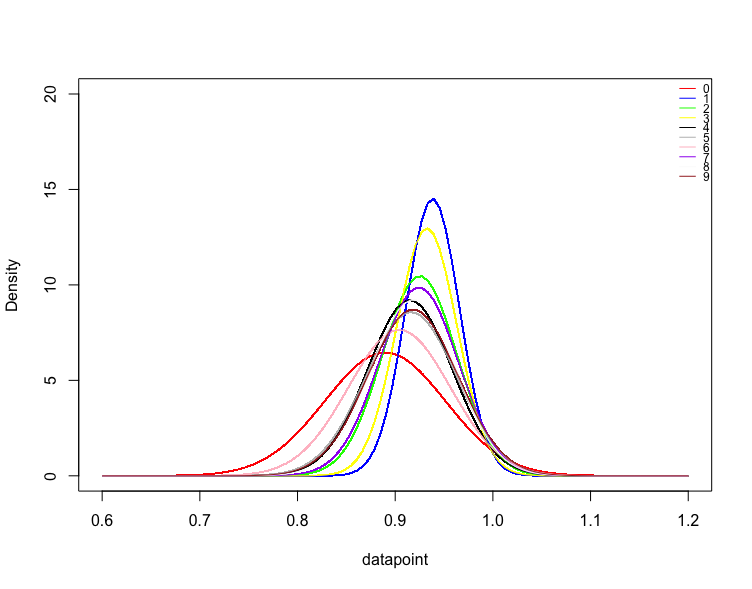
\includegraphics[width =  \textwidth]{ndist_muld_class.png}
\end{figure} 

It seems the like the space which the digit number 1 resides in has a very high density, which could explain why most of the predicition which were found went towards that value. 
Other than that, it also shows that the class is in general is pretty interlapped with each other, which indicate that the method itself might not be that suitable for this type of problem.  The method seems based from figure \ref{fig:false_g_g} better or more accurate at smaller dataset than bigger dataset. 

\subsection{PCA-based binning}
An alternative method to binning based on direct pixel feature descriptors was applied.
This method consisted of preprocessing the smoothed (gaussian blur with \(\sigma=0.6\))
and downsampled (100 DPI) data through Principal Component Analysis (PCA).

This method was used to investigate:
\begin{itemize}
\item The effect of the Laplace correction.
\item The difference between using a Normal probability density function estimator vs. Kernel density estimation.
\item An optimal PCA threshold for proportion of cumulative variance explained for this method.
\end{itemize}

Figure \ref{fig:nbPDresults} shows the accuracy
of the Naïve Bayes classifier applied to the PCA-processed data
with four different parameter setups.

\begin{figure}[ht]
\centering
\includegraphics[width=0.9\textwidth]{nbPD-accuracy-vs-pca-vs-nb.eps}
\caption{Accuracy vs. PCA threshold vs. Naïve Bayes method parameters.
The G2M2 dataset with 4000 hand written digits was used.}
\label{fig:nbPDresults}
\end{figure}

Figure \ref{fig:nbPDresults} clearly shows
that the choice of PCA threshold matters, and that the threshold
should be selected around 80 \%.
It is also seen that the Laplace correction has no noticeable effect.
This is probably due to the nature of the principal components,
which are linear combinations of the actual pixel intensities,
and them being representatives of data variance.
Lastly, it is seen that the Kernel Density Estimation (KDE) method
yields slightly better accuracies than the Normal distribution method.
This result is likely due to the data not being entirely normally distributed.

The most noticable traits of this PCA-based method are that
it reduces data processing time, as shown in previous exercies,
and that the obtained accuracies are significantly higher than
when using the direct pixel-based binning method.
In agreement with the results of the other method,
when the number of bins was increased to near-maximum values (324 pixels / principal components),
the classification performance deteriorated.

\end{document}